When studying temporal structures in neural dynamics, the definition of the time references is a key first point. In the computational analysis in the previous section, the time reference to define the intervals where first and last spike in the burts. In that case, as well as in the case of inter-neurons in \textit{C. maenas} the CPG phases are directly related with the bursting activity of these neurons. However, in the case of \textit{Lymnaea stagnalis}, activity is usually characterized using recordings from both inter-neurons and moto-neurons \parencite{elliot, benjamin, crossley}. This leads to a more flexible reference of the time references, so for this analysis, references will be defined by the phase and each phase will be bounded by different neurons. For example, in Figure \ref{fig:example lymnaea phases recording} the three phases in the  CPG are marked over the recording, note how it can be delimited by the neurons in the circuit but some of the moto-neurons cover several phases and that phases are delimited not only by the spikes but the hyperpolarization periods. Therefore, to characterize the time sequences in the feeding CPG, we need compound reference from several neural recordings that can be summarized as in Table \ref{table:cpg ref intervals}

%\TODO revisar
Table \ref{table:tabla spikes} displays a summary of some neurons involved in each phase. \todo{viene del tfm revisar}

% Please add the following required packages to your document preamble:
% \usepackage{multirow}
\begin{table}[htb!]
	\begin{tabular}{cl|l|ll}
		\multicolumn{1}{l}{}                                 & \multicolumn{1}{c|}{\textbf{N1}} & \multicolumn{1}{c|}{\textbf{N2}} & \multicolumn{1}{c}{\textbf{N3}} &  \\
		\multicolumn{1}{c|}{\multirow{2}{*}{\textbf{Start}}} & Last spike of N3t/B3             & Inhibition of B5                 & First spike of B8               &  \\
		\multicolumn{1}{c|}{}                                & Depolarization in B1             &                                  &                                 &  \\ \cline{1-4}
		\multicolumn{1}{c|}{\multirow{2}{*}{\textbf{End}}}   & Last spike of B5                 & First spike of B8                & Last spike of N3t/B3            &  \\
		\multicolumn{1}{c|}{}                                & Hyperpolarization in B1          &                                  &                                 & 
	\end{tabular}
	\caption{Time reference boundaries for the three phases in the feeding CPG}
	\label{table:cpg ref intervals}
\end{table}


\begin{table}[h!]
	\centering
	\begin{tabular}{lccc}
		Neuron                                           & \multicolumn{1}{l}{Protraction} & \multicolumn{1}{l}{Rasp} & \multicolumn{1}{l}{Swallow} \\ \hline
		Interneuron                                     & N1                              & N2                       & N3                          \\
		& \multicolumn{1}{l}{}            & \multicolumn{1}{l}{}     & \multicolumn{1}{l}{}        \\
		\multicolumn{1}{c}{\multirow{3}{*}{Motoneuron}} & B7                              & B10                      & B3                        \\
		\multicolumn{1}{c}{}                            & B6                              & B4                       & B9                        \\
		\multicolumn{1}{c}{}                            & B1                              &                          &                         
	\end{tabular}
	\caption{Neuron participation in feeding phases.}
	\label{table:tabla spikes}
\end{table}



\begin{figure}[bth!]
\centering
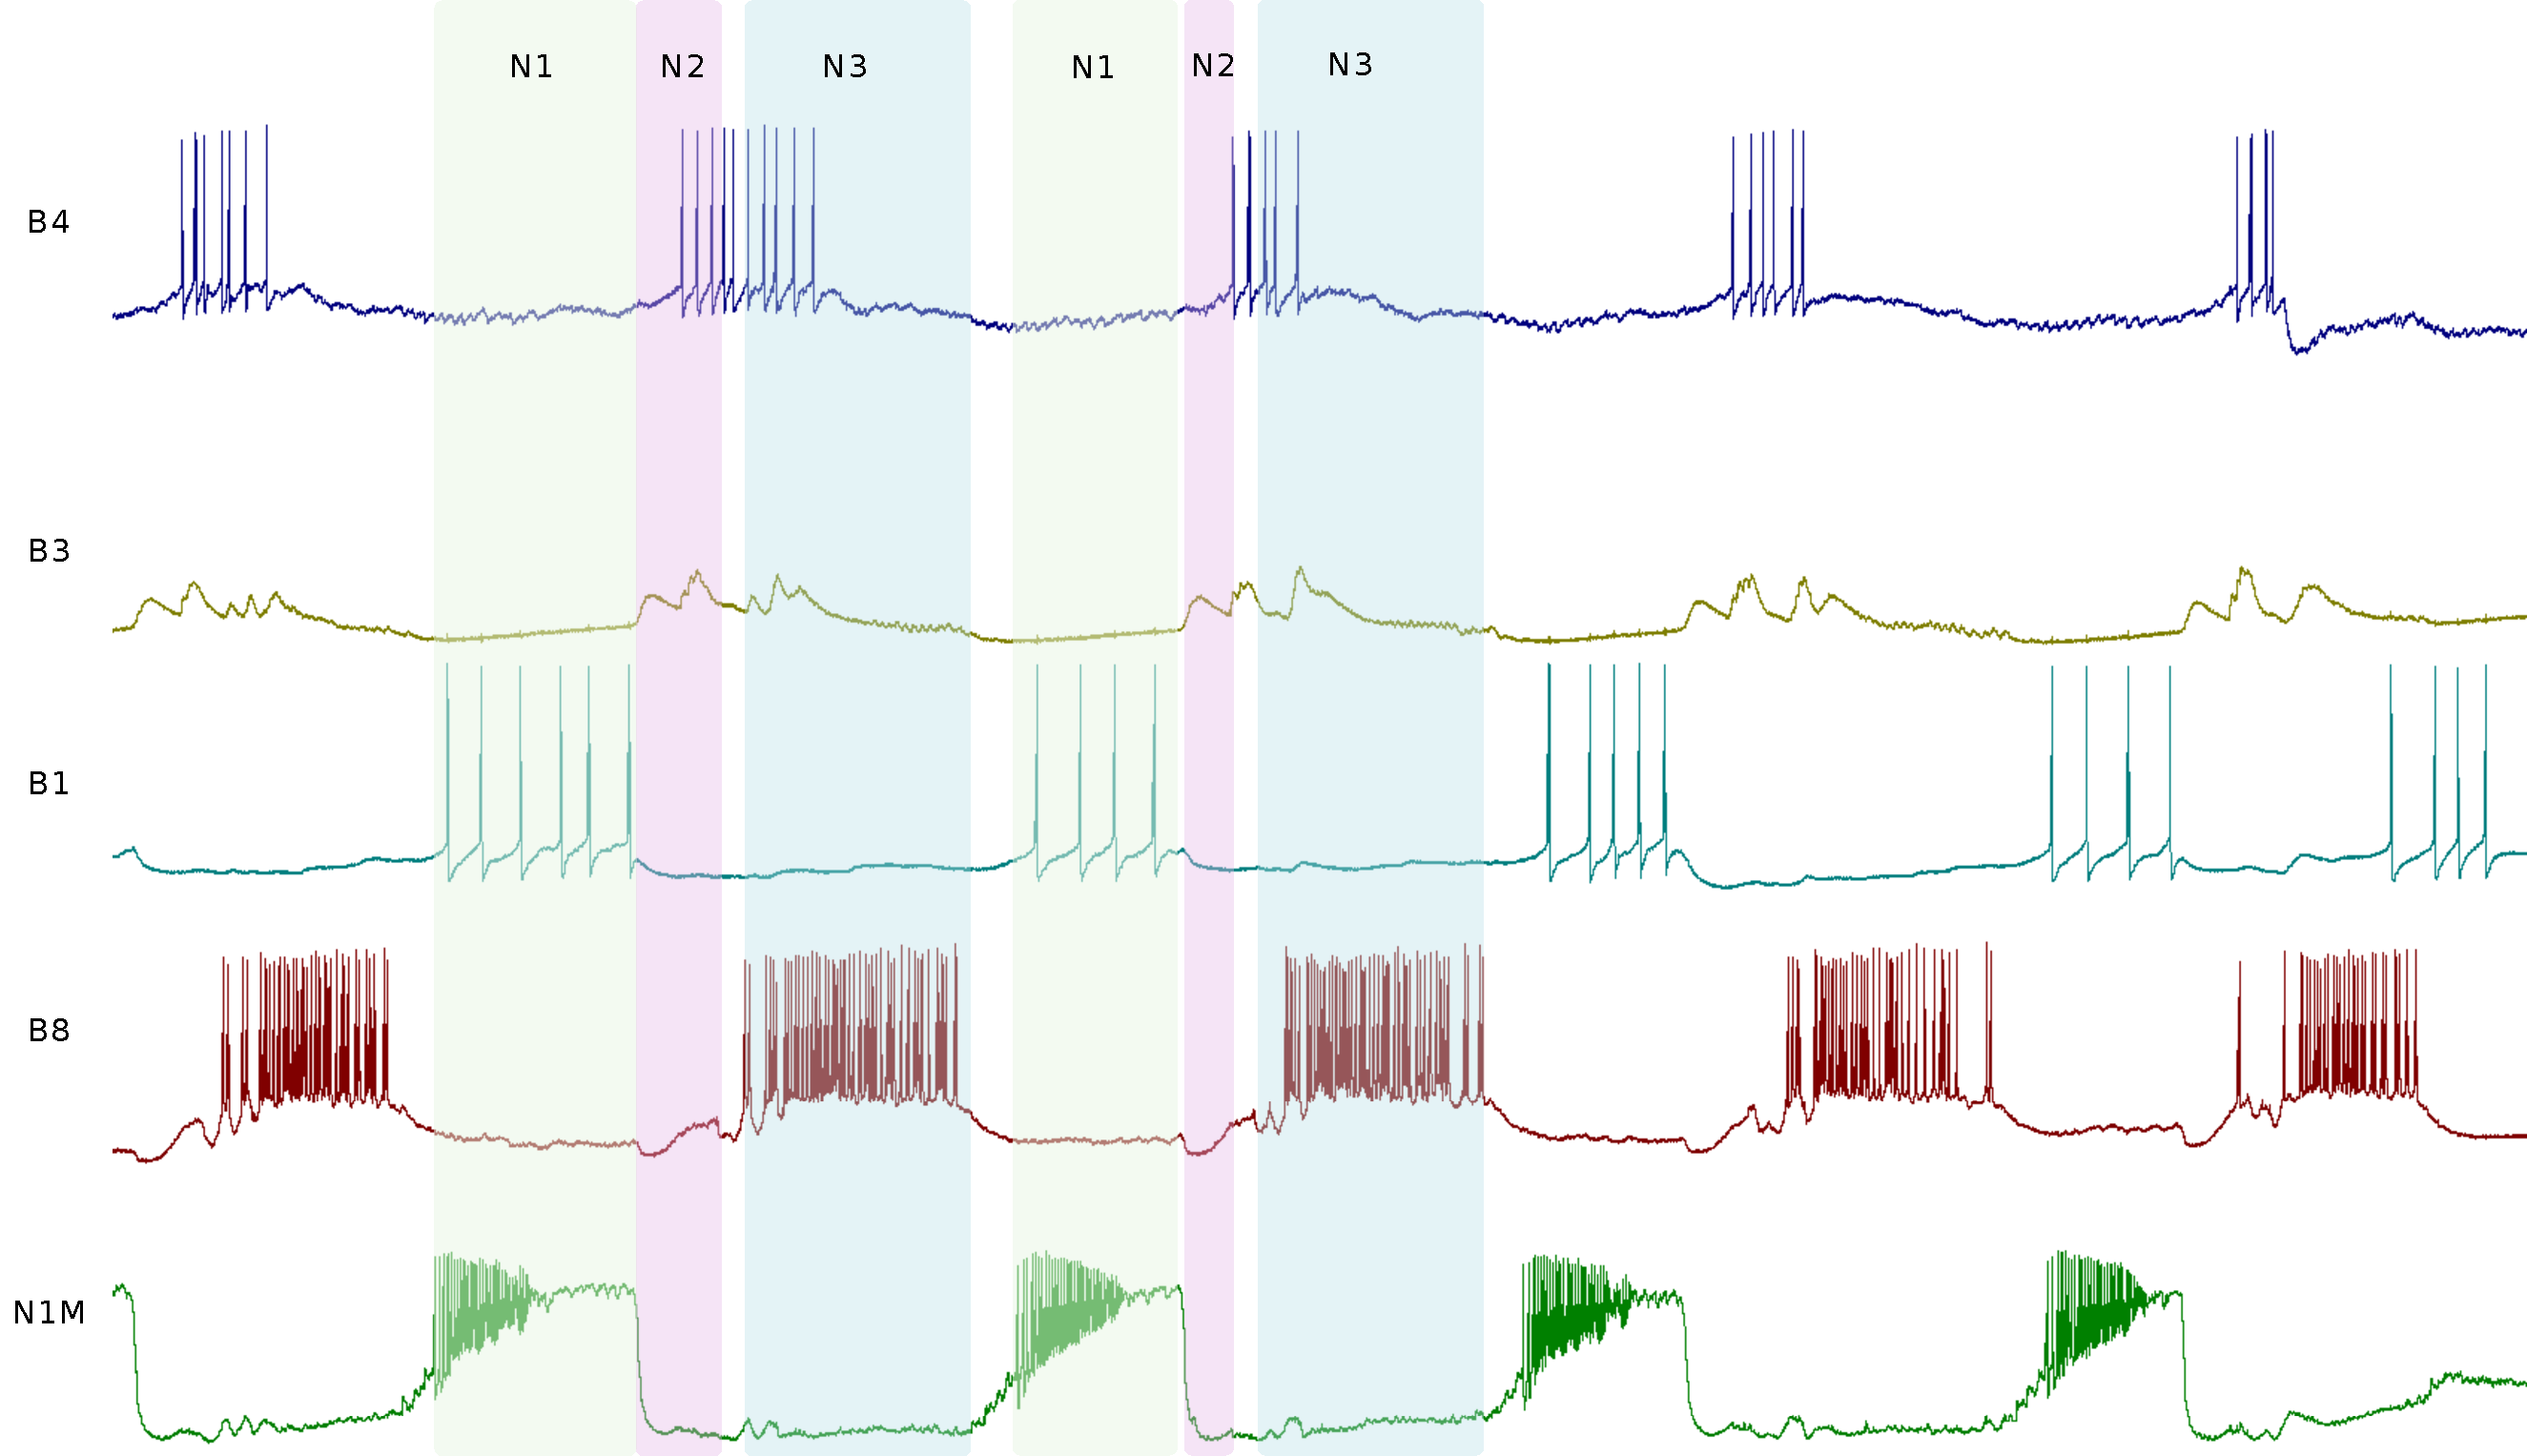
\includegraphics[width=\textwidth]{img/invariants/example_phases_1.pdf}
\\
\vspace{10pt}
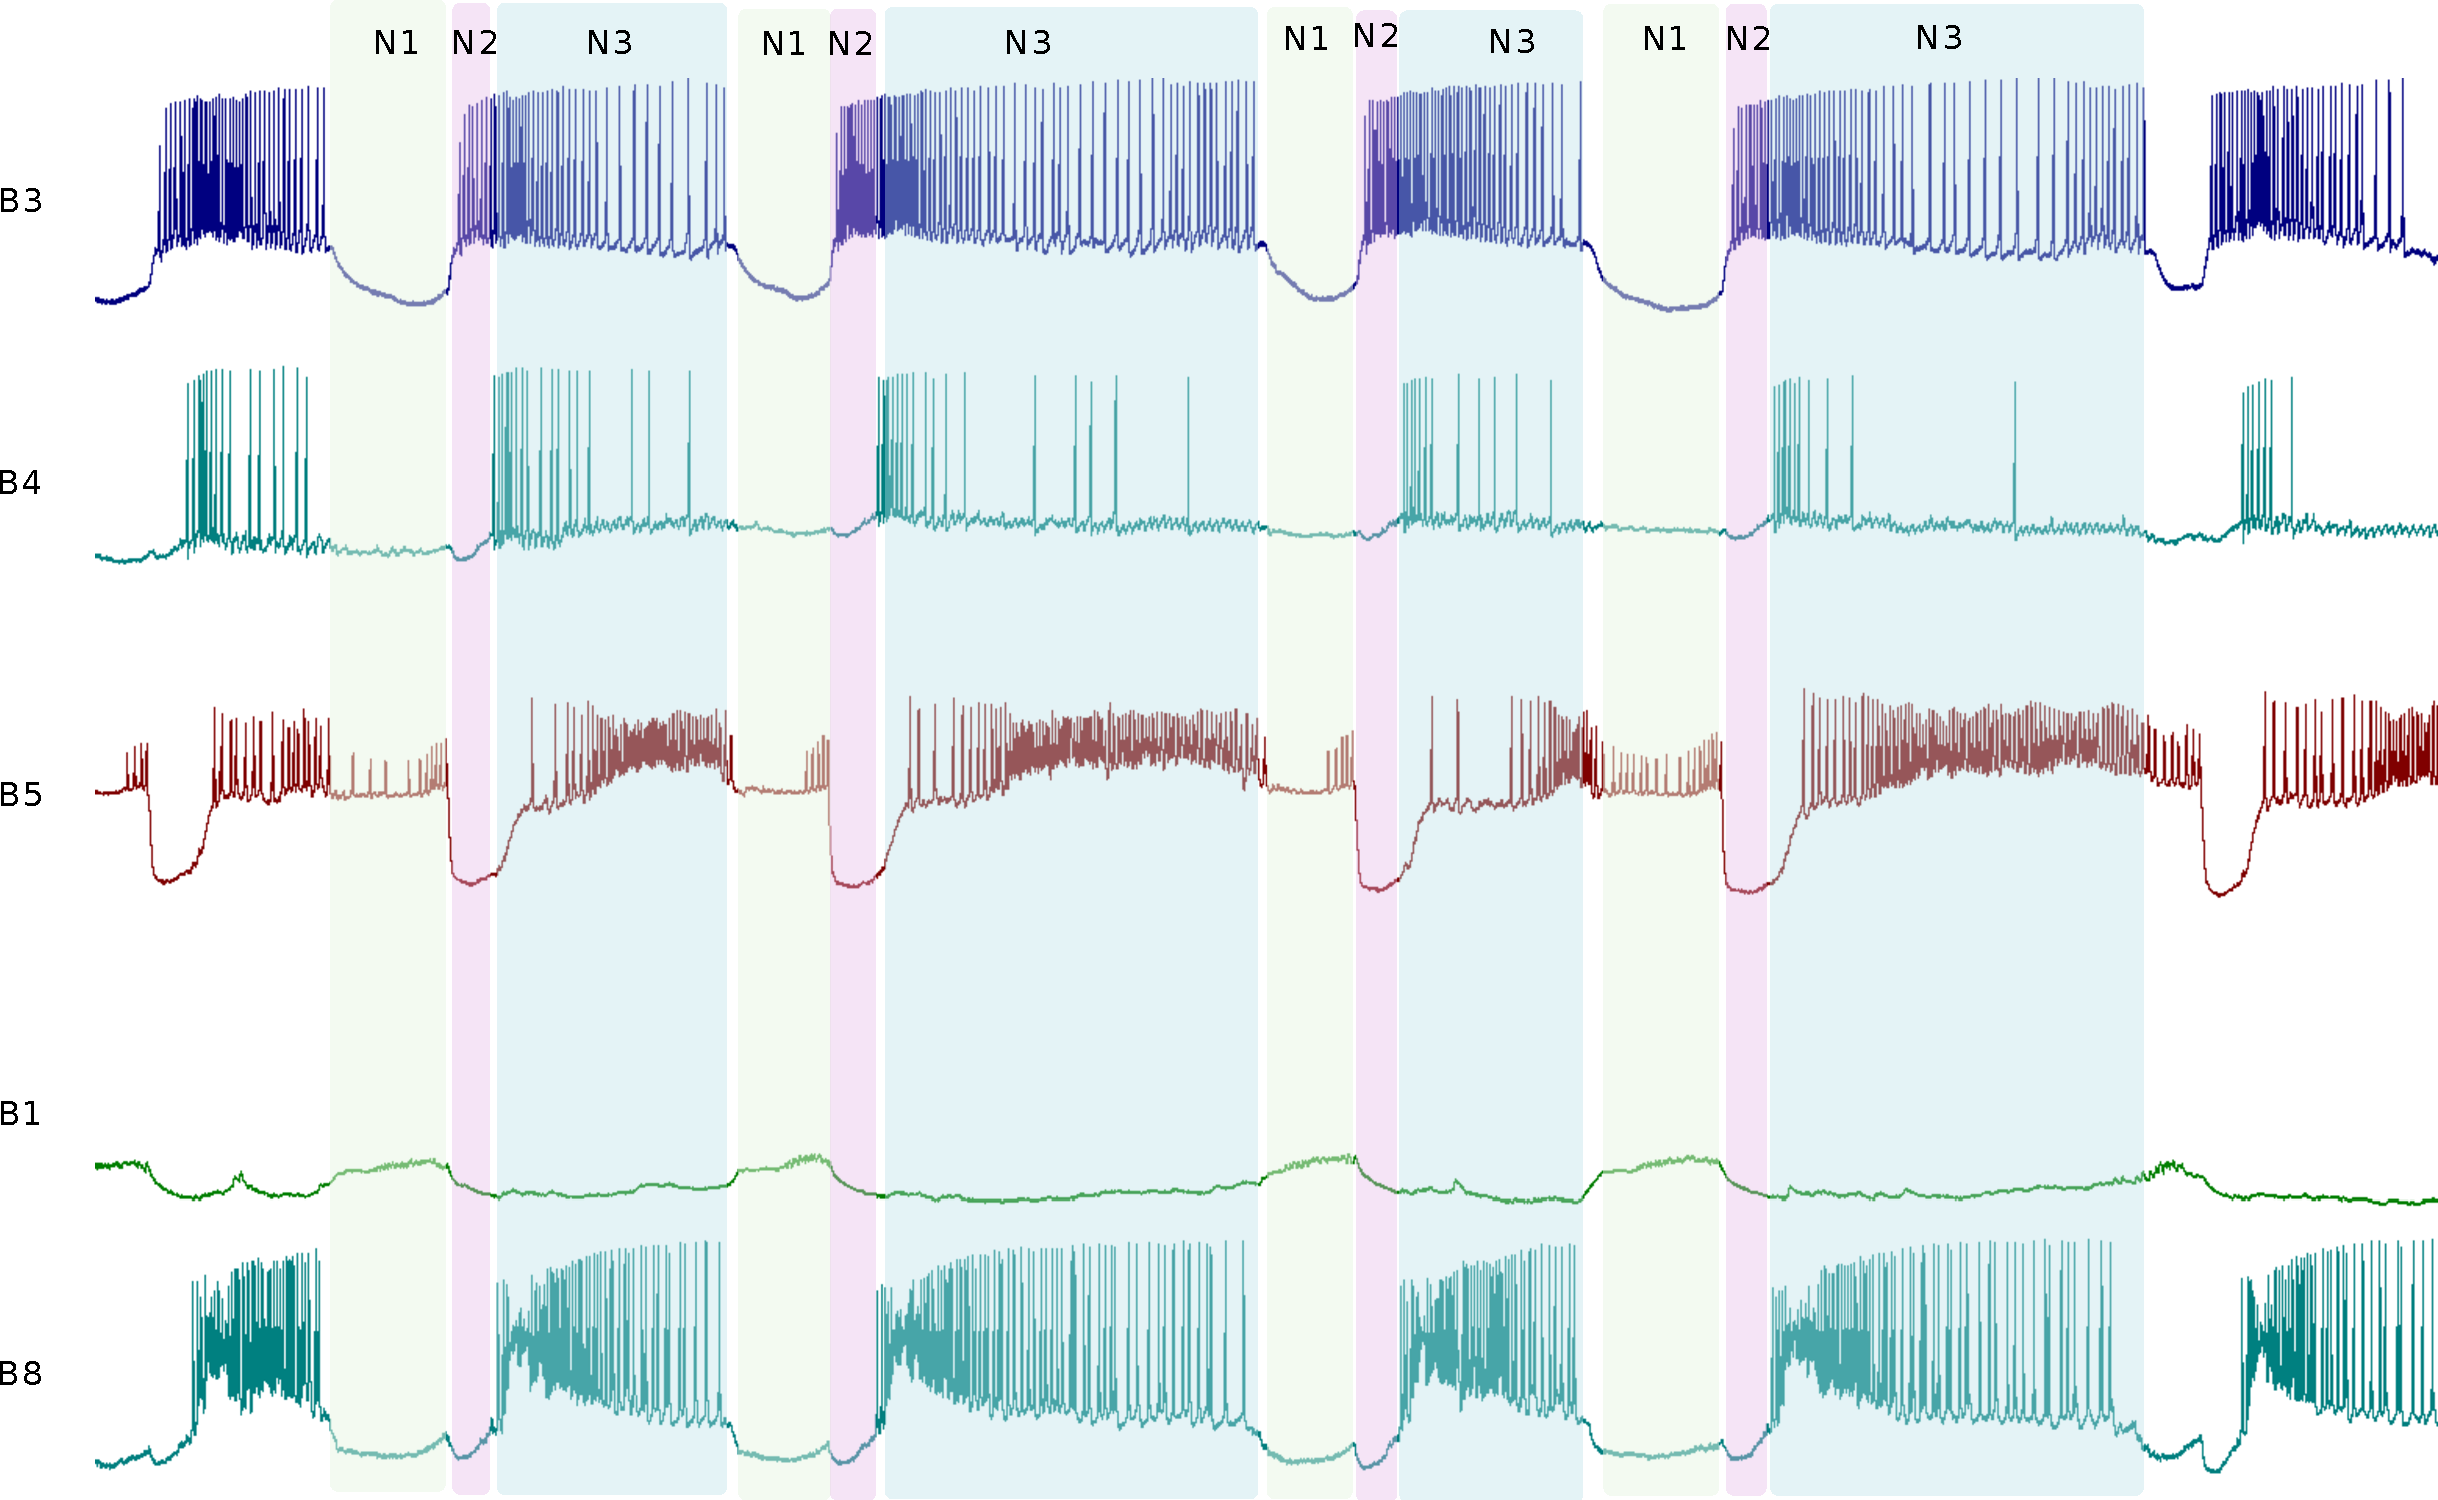
\includegraphics[width=\textwidth]{img/invariants/example_phases_2.pdf}
\caption{Delimitation of phases in the feeding CPG of \textit{Lymnaea stagnalis} based on different recordings.}
\label{fig:example lymnaea phases recording}
\end{figure}



\subsubsection{Invariants in spontaneous activity}



\begin{figure}[bth!]
	\centering
	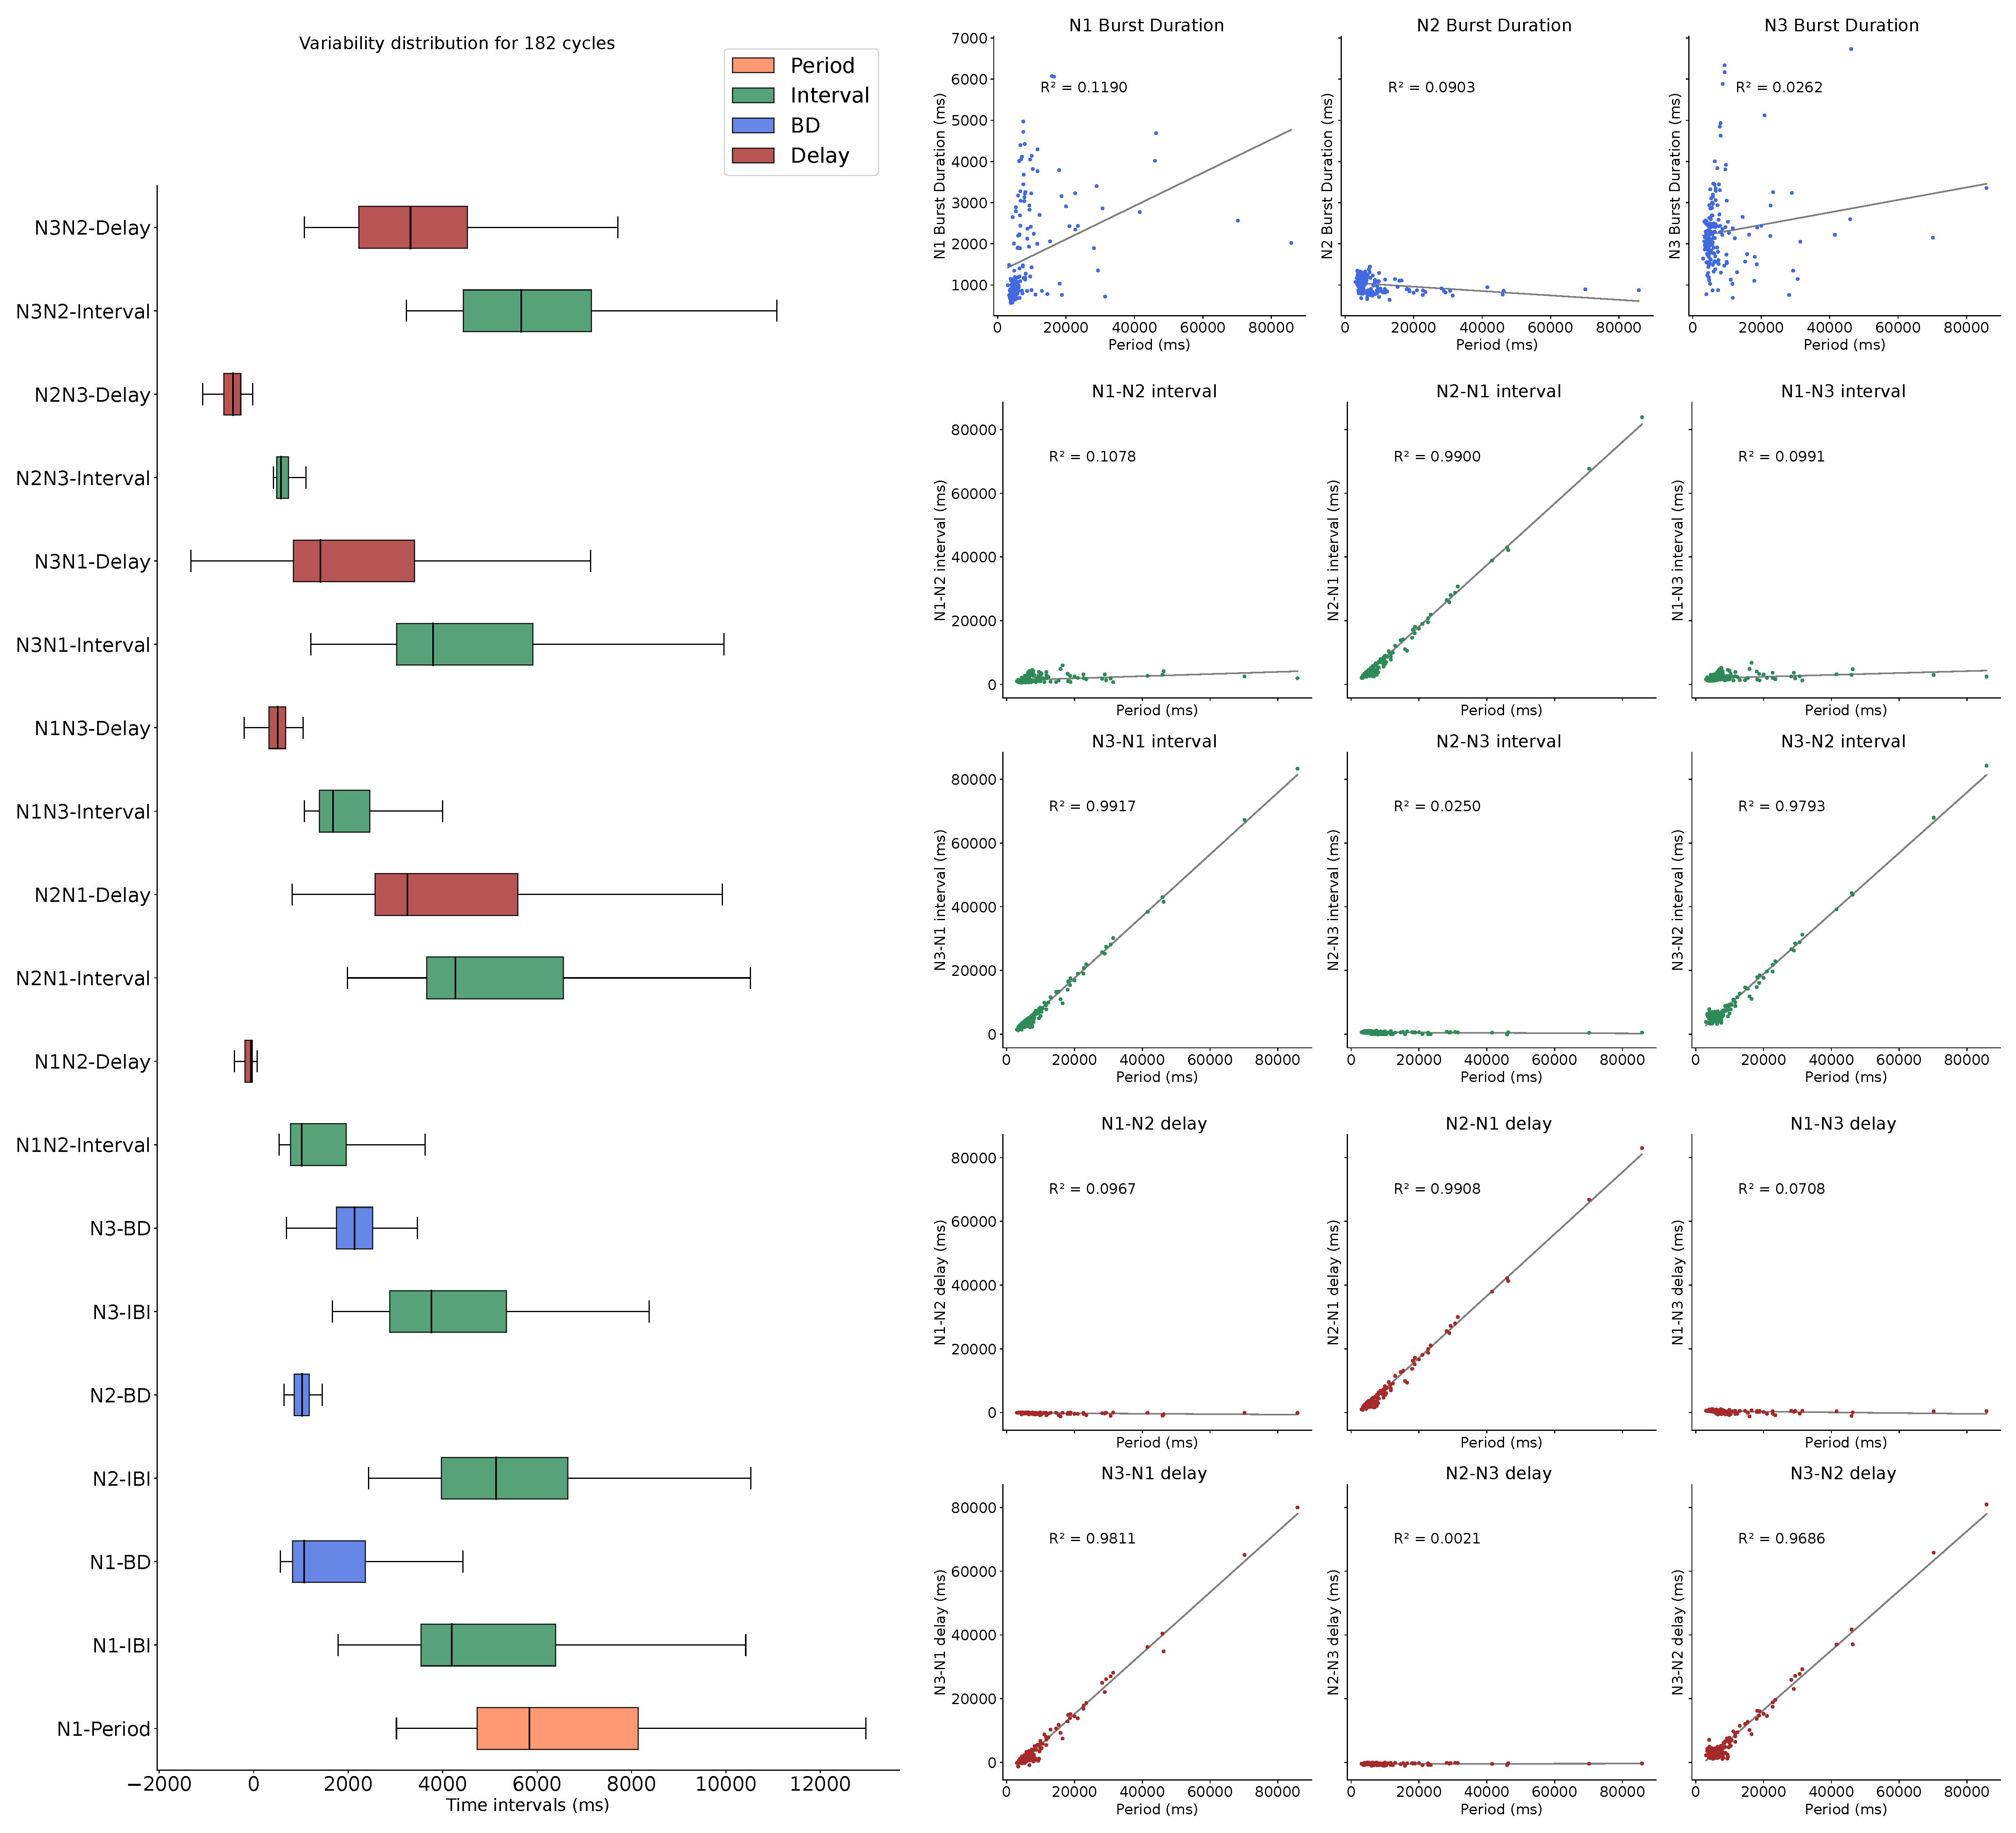
\includegraphics[width=\textwidth]{img/invariants/prep1_3 intervals panel.pdf}
	\caption{Boxplots and correlation of main intervals in spontaneous activity of \textit{L. stagnalis}}
	\label{fig:prep1 invariants}
\end{figure}



\begin{figure}[bth!]
	\centering
	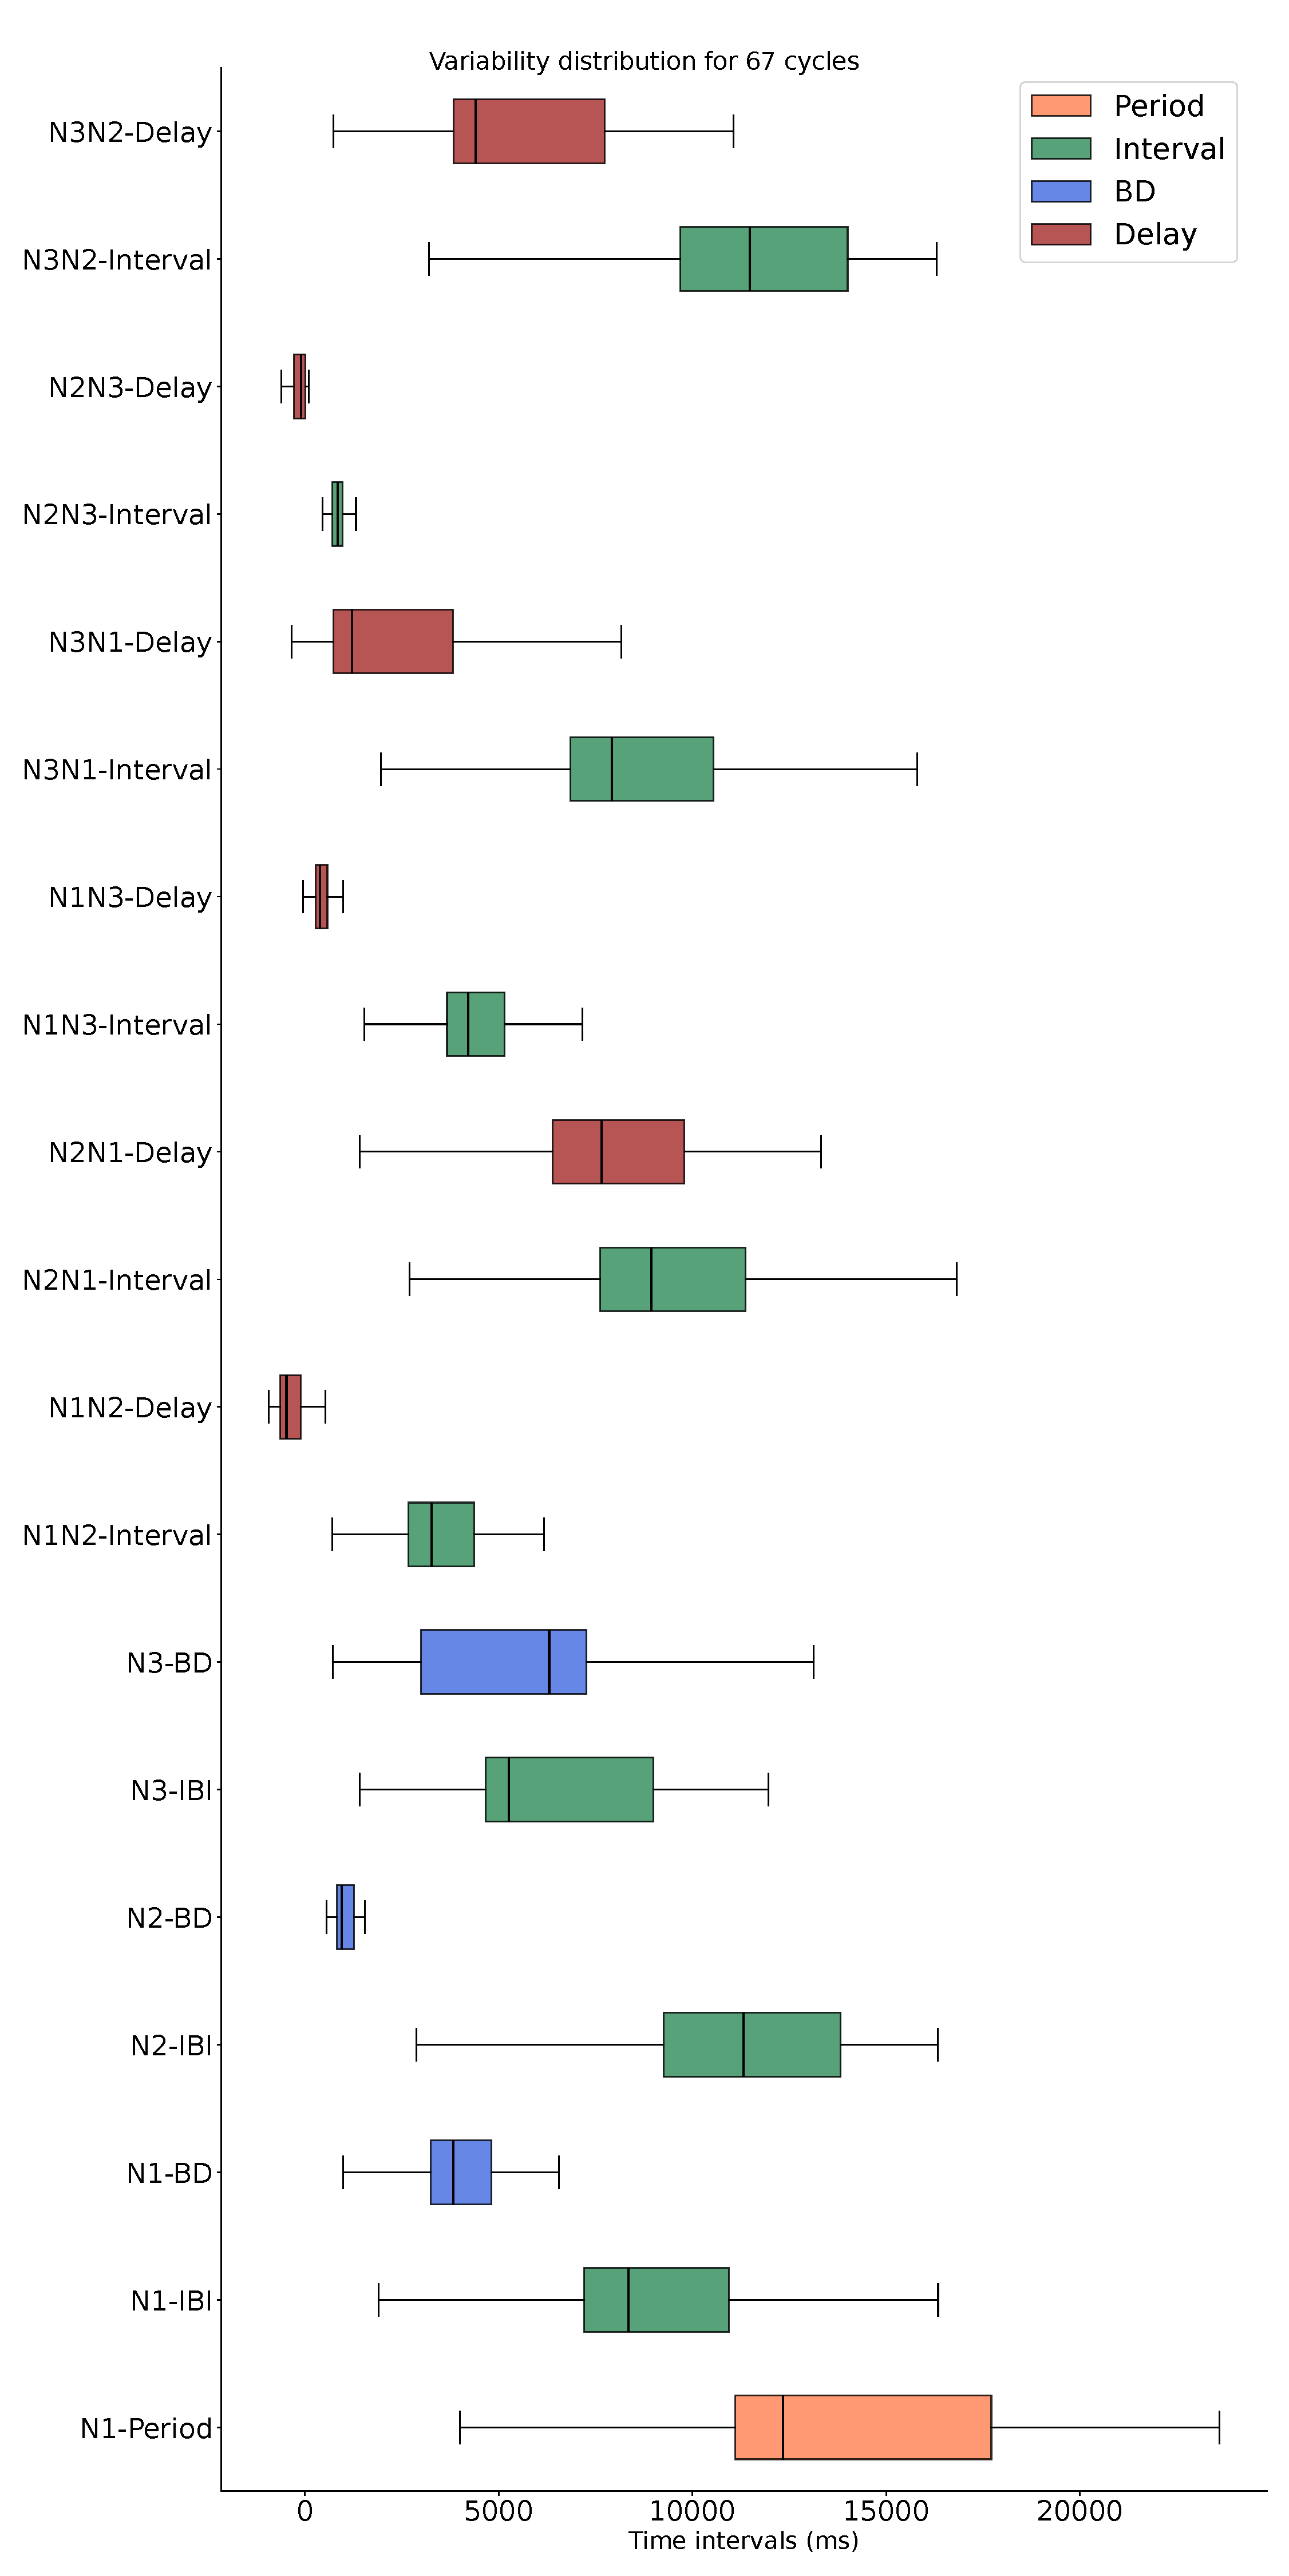
\includegraphics[width=\textwidth]{img/invariants/prep3_3 intervals panel.pdf}
	\caption{Boxplots and correlation of main intervals in spontaneous activity of \textit{L. stagnalis}}
	\label{fig:prep3 invariants}
\end{figure}




\subsubsection{Invariants in SO driven activity}
\large{spontaneous driven}
% Nota: datos de preparación 4 en la detección está solo n1m y b8, las fases son N1 y N3. 
 
 	
 	
\begin{figure}[bth!]
	\centering
	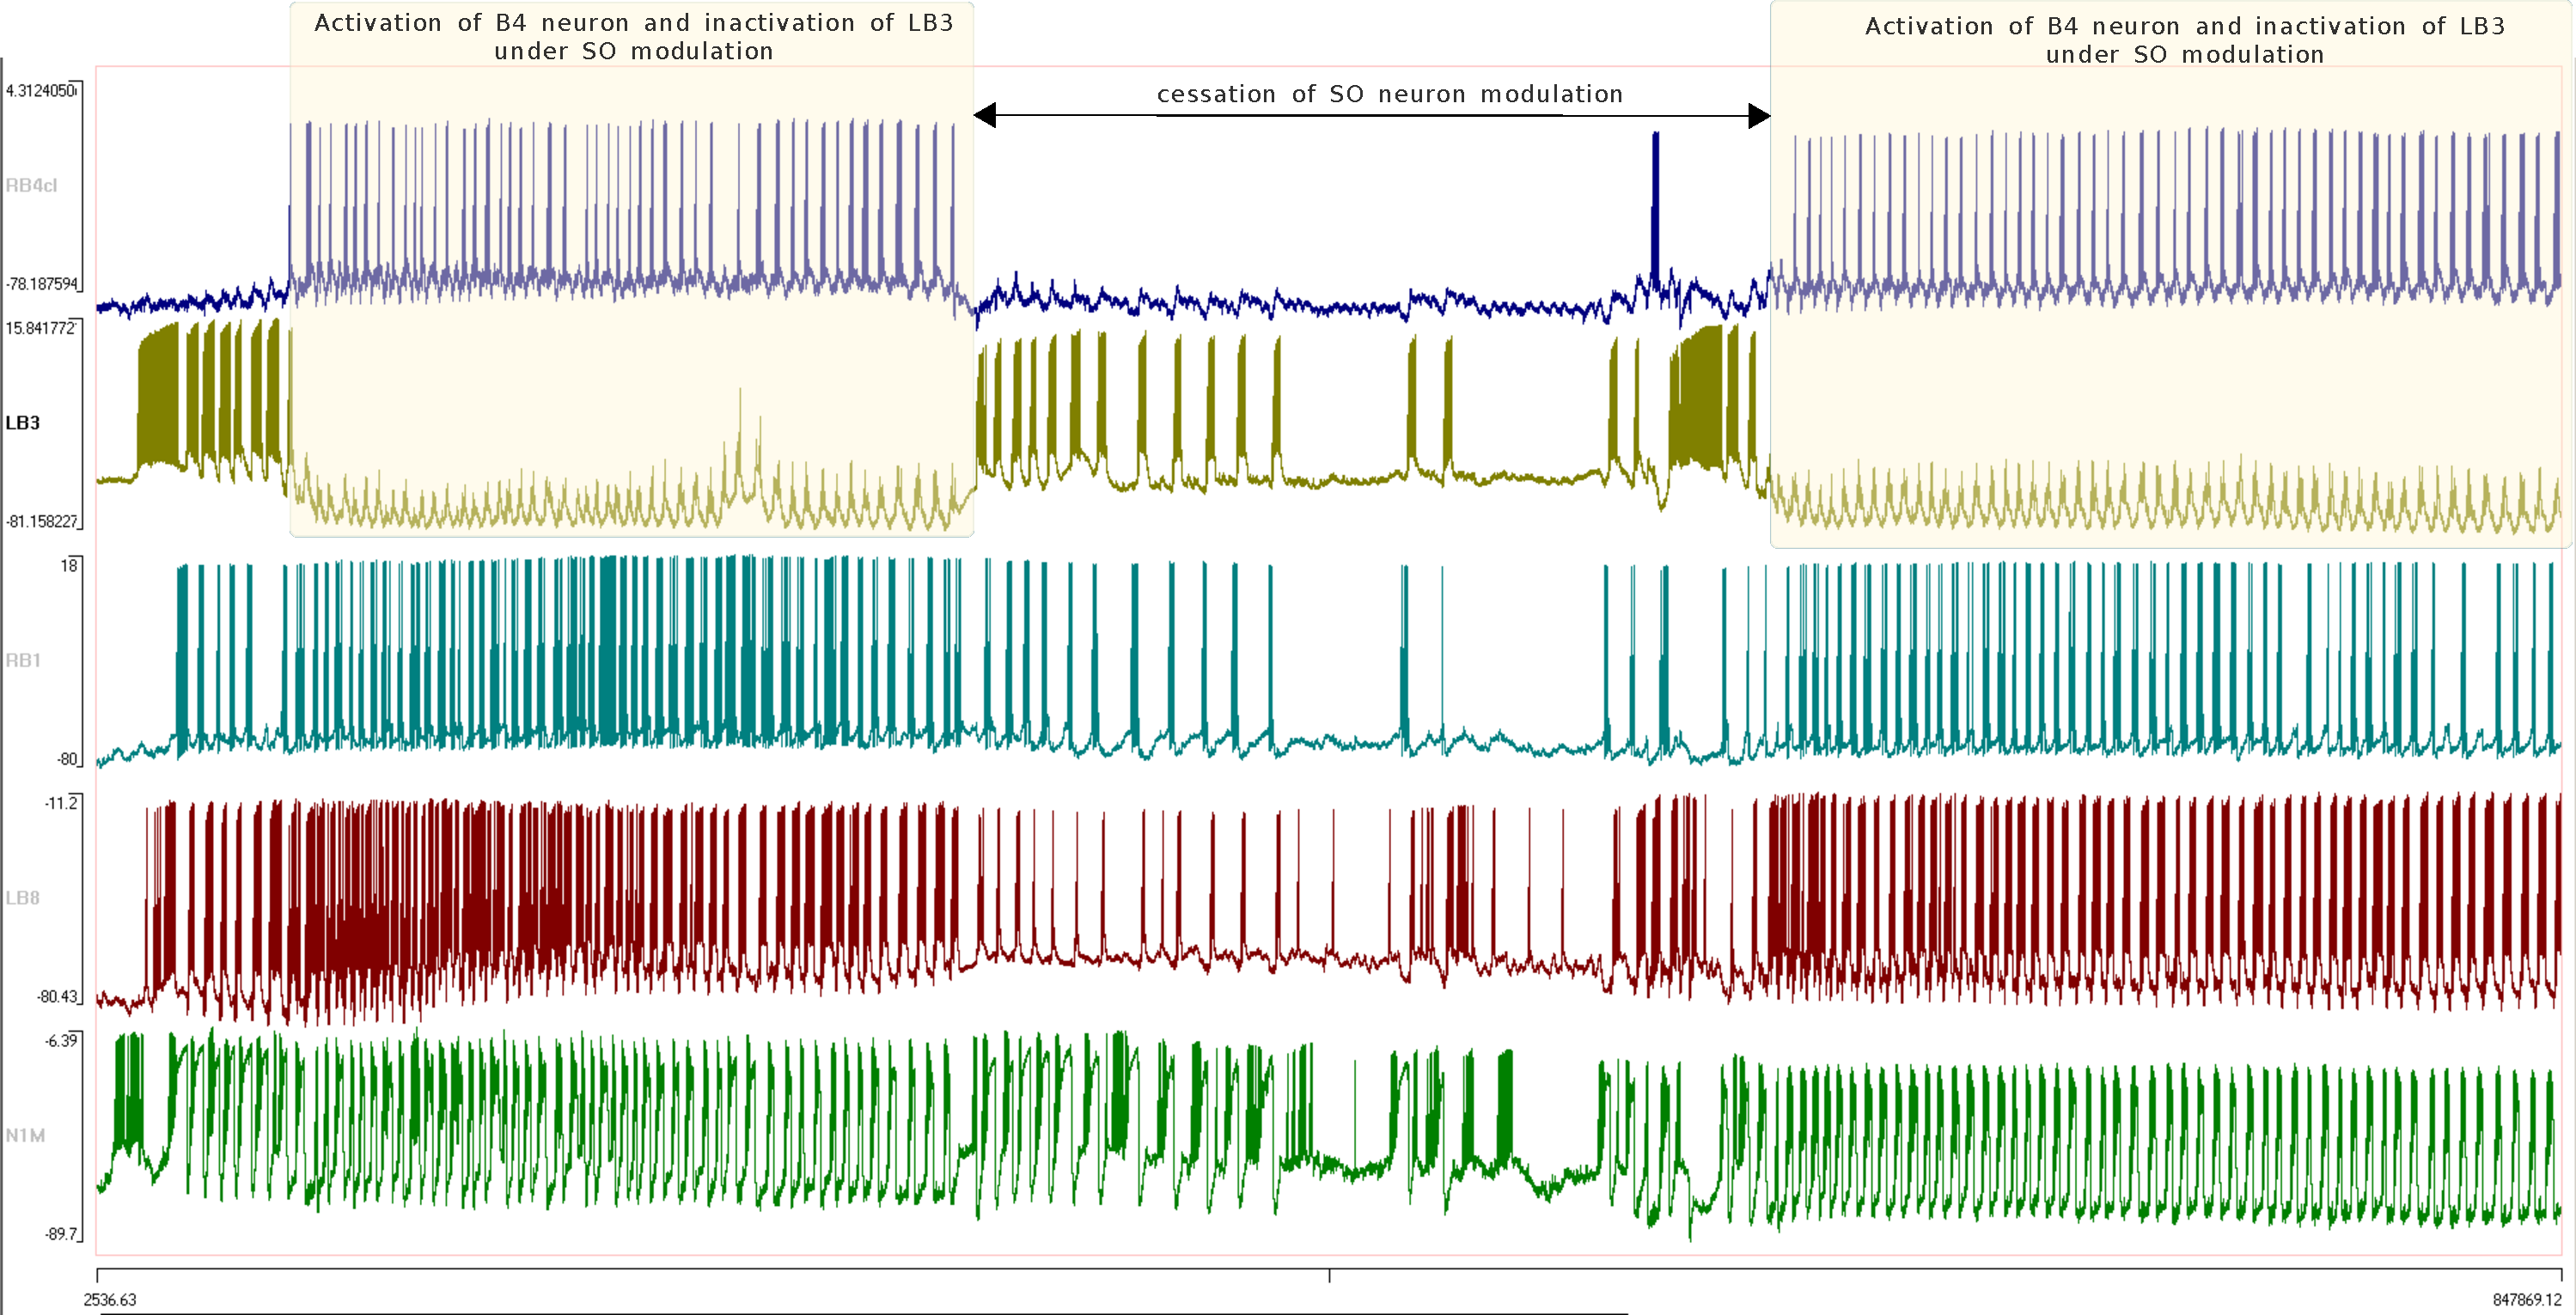
\includegraphics[width=\textwidth]{img/invariants/SO-spontaneuous-driven.pdf}
	\caption{Example of the CPG activity when the SO neuron is driven the rhythm}
	\label{fig:SO-spontaneuous-driven}
\end{figure}




\begin{figure}[bth!]
	\centering
	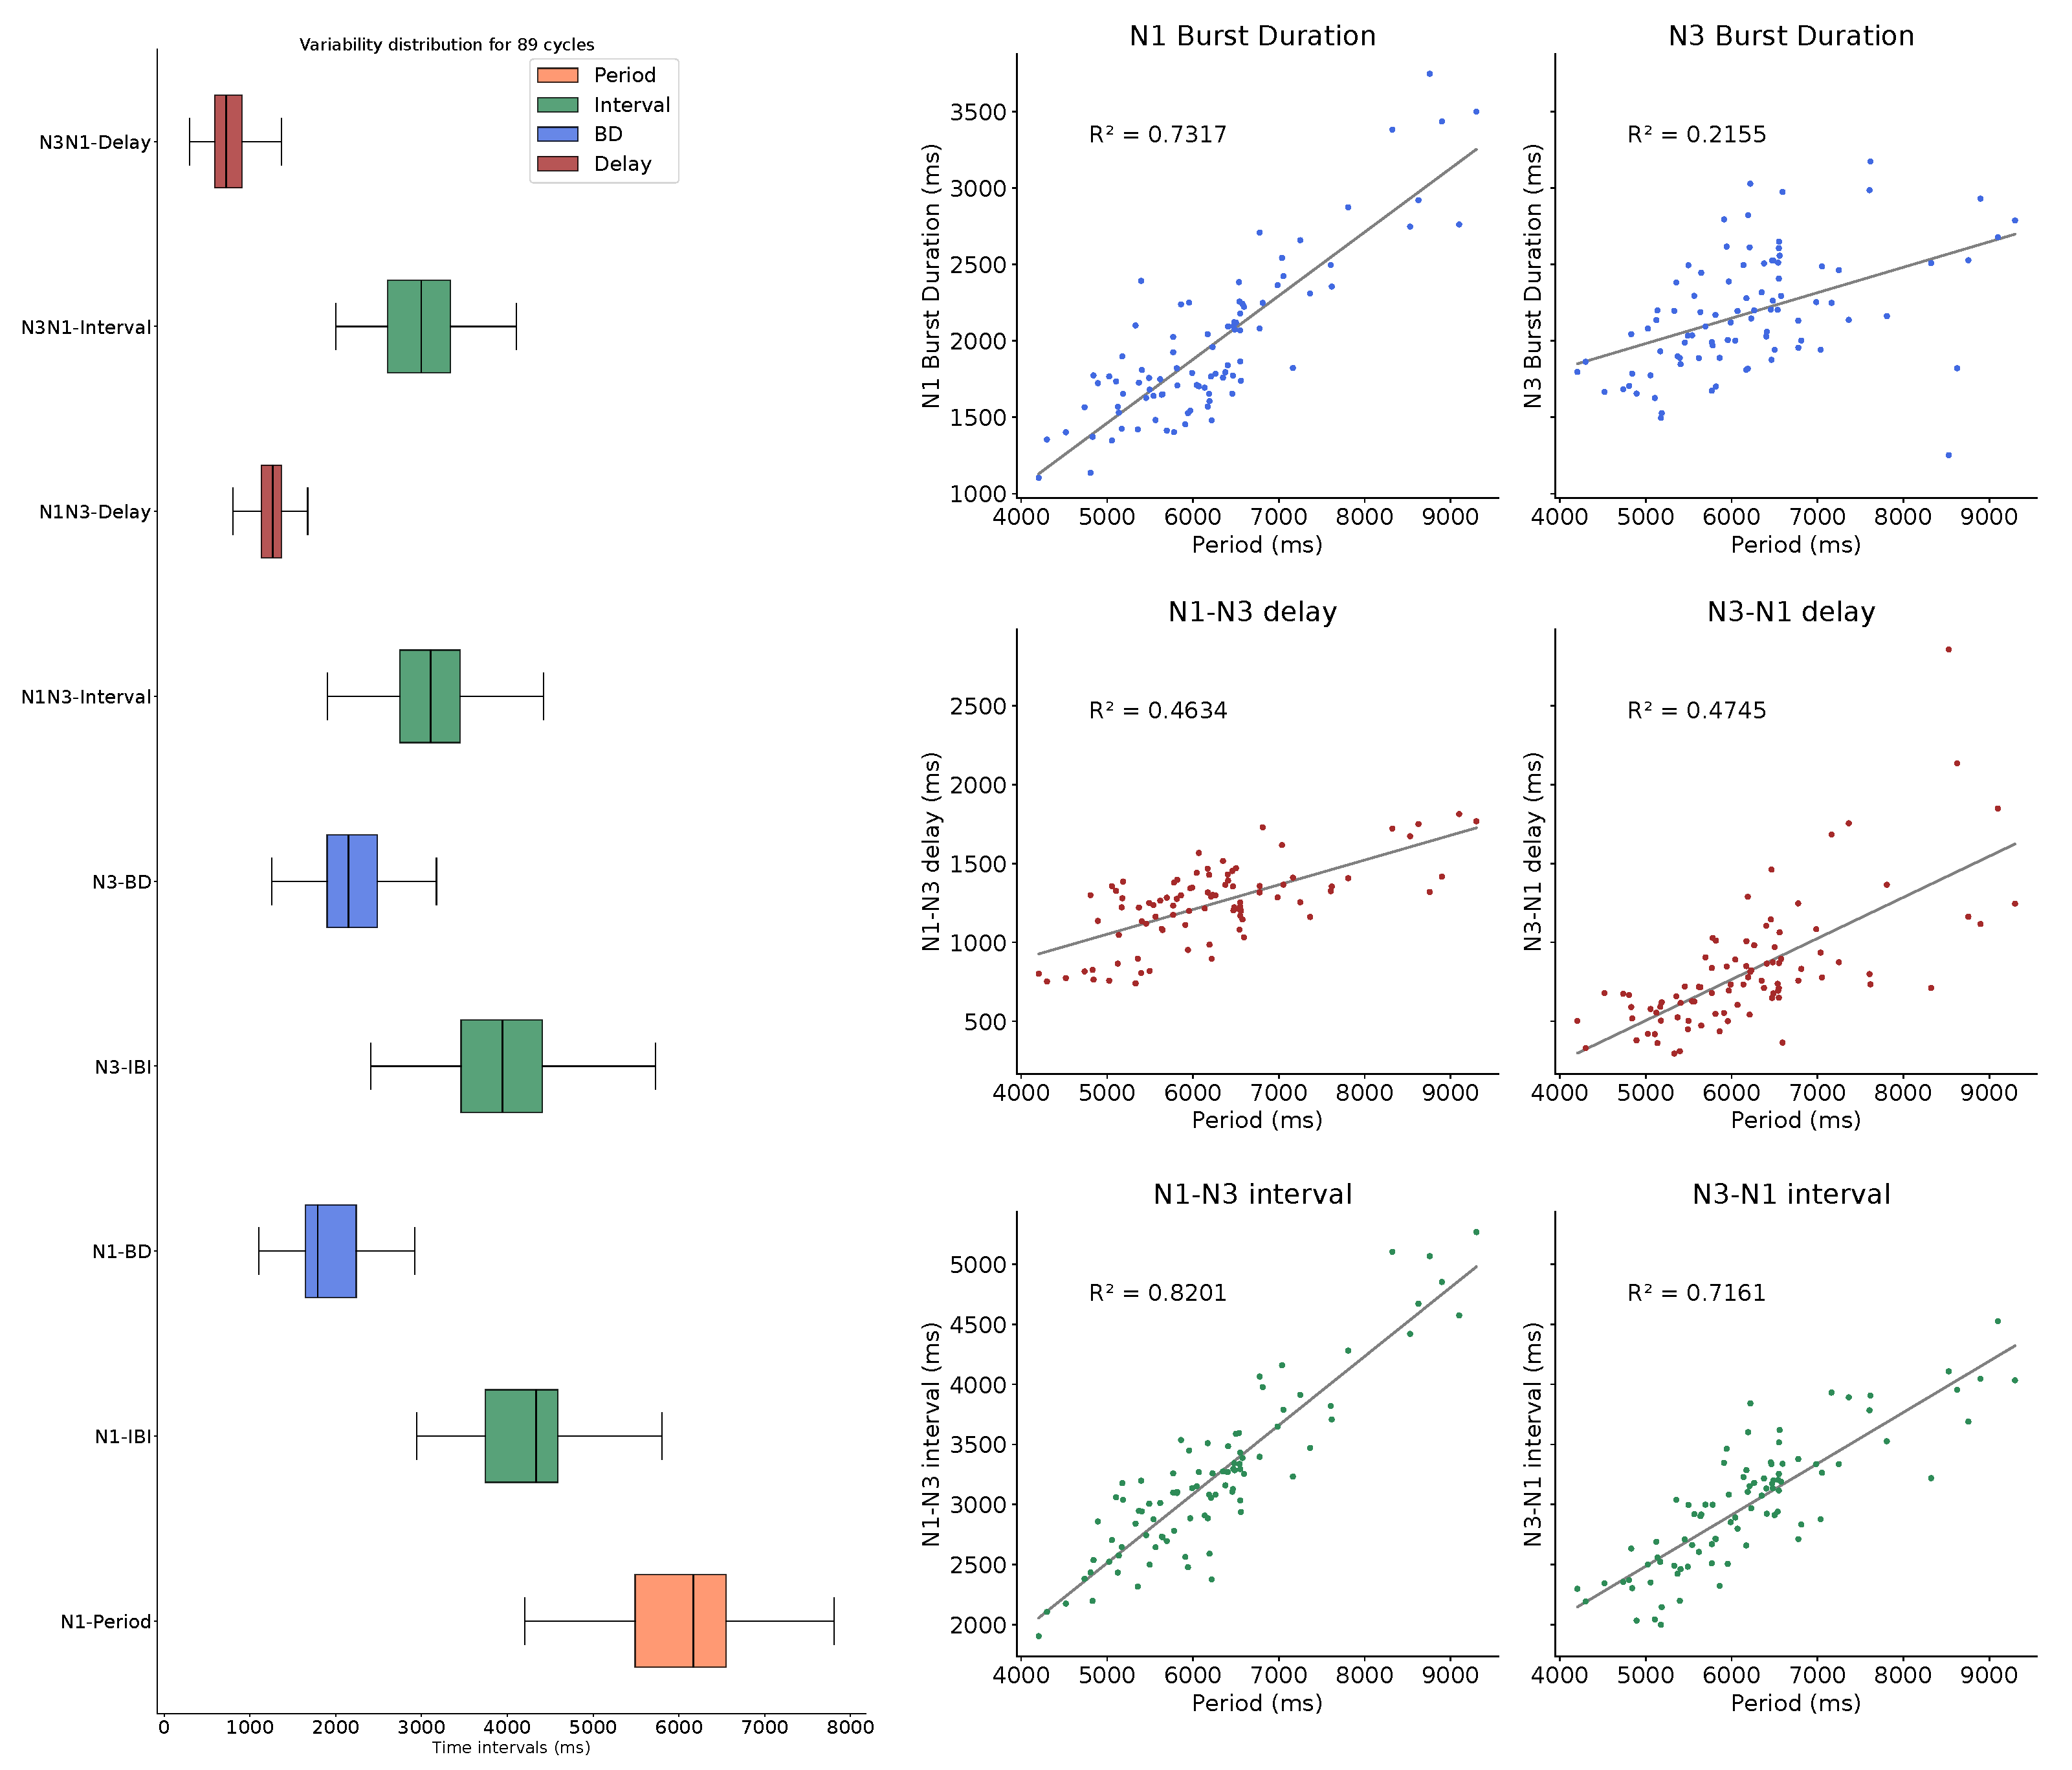
\includegraphics[width=\textwidth]{img/invariants/prep4_so_driven_2 intervals panel.pdf}
	\caption{Boxplots and correlation of main intervals in spontaneous activity of \textit{L. stagnalis} during SO modulation}
	\label{fig:prep4 so driven invariants}
\end{figure}
 	
 
 
\large{stimulated driven}


\subsubsection{Invariants in MLN stimulation driven activity}
The snail's lips are connected to the cerebral ganglia by the MLN (median lip nerves). It is possible to stimulate CPG activity by its stimulation, simulating the initiation of the rhythm in food presence \parencite{staras_electrophysiological_2019}. The data in this recording was stimulated by (4volt 1Hz stim).






\subsubsection{Invariants in cv1 stimulation driven activity}